\chapter{Entwicklung des Prototpys für IntelliJ}
\label{cha:EntwicklungIntelliJ}

\section{Design}
\label{sec:EntwicklungIntelliJ_Design}


\begin{figure}
    \centering
    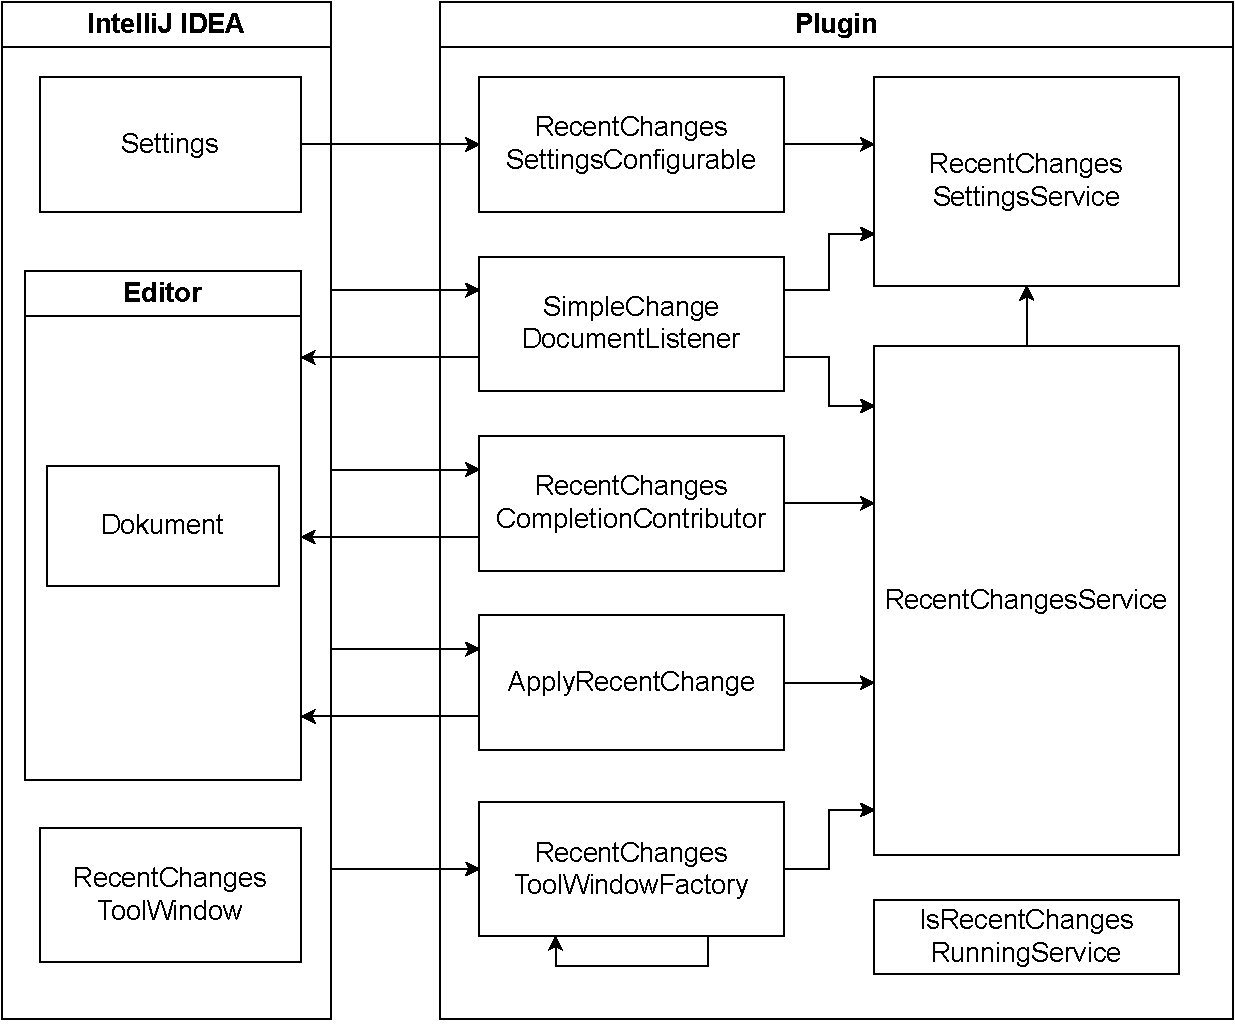
\includegraphics[width=.95\textwidth]{diagram_IntelliJDesign-Simplified}
    \caption{Stark vereinfachte Übersicht über das Design des Plugins in IntelliJ.}
    \label{fig:diagram_IntelliJDesign-Simplified}
\end{figure}   
\begin{figure}
    \centering
    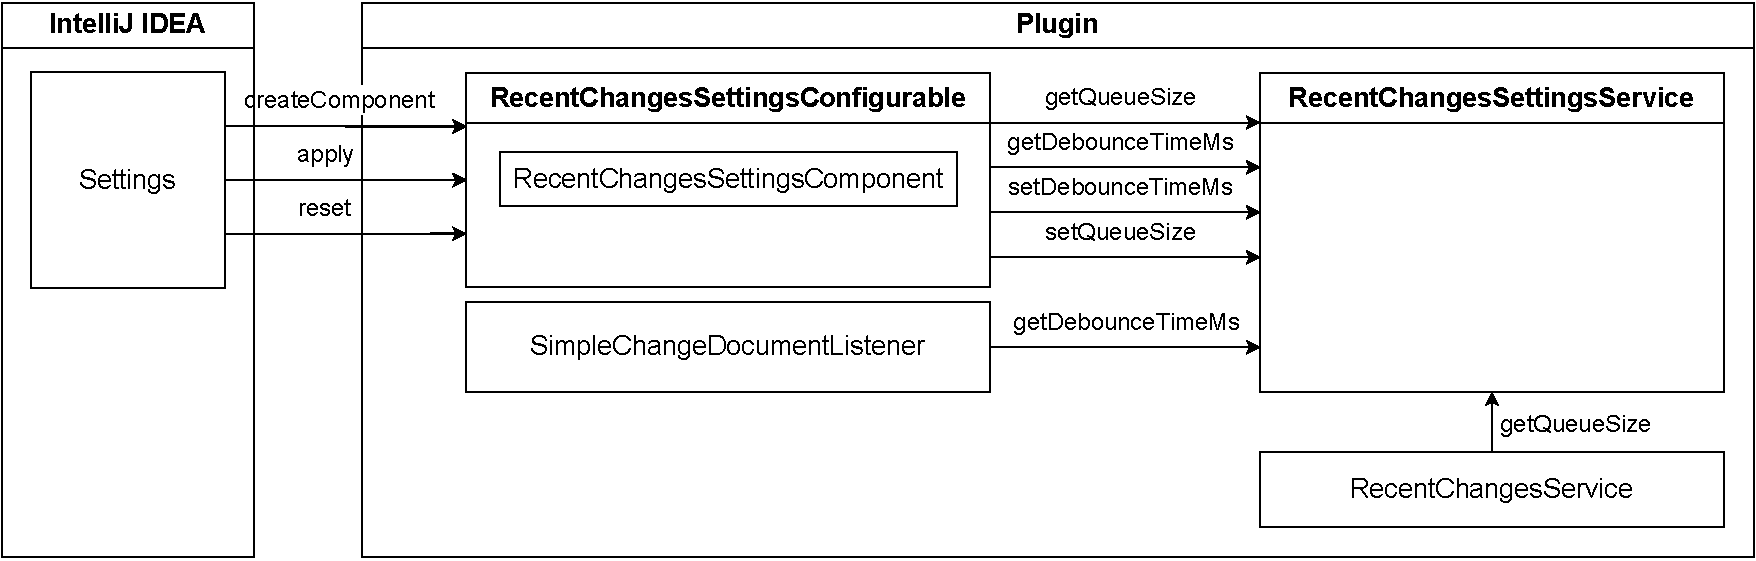
\includegraphics[width=.95\textwidth]{diagram_IntelliJDesign-Detail_Settings}
    \caption{Detaillierte Darstellung der \emph{Settings} Komponenten.}
    \label{fig:diagram_IntelliJDesign-Detail_Settings}
\end{figure}   
\begin{figure}
    \centering
    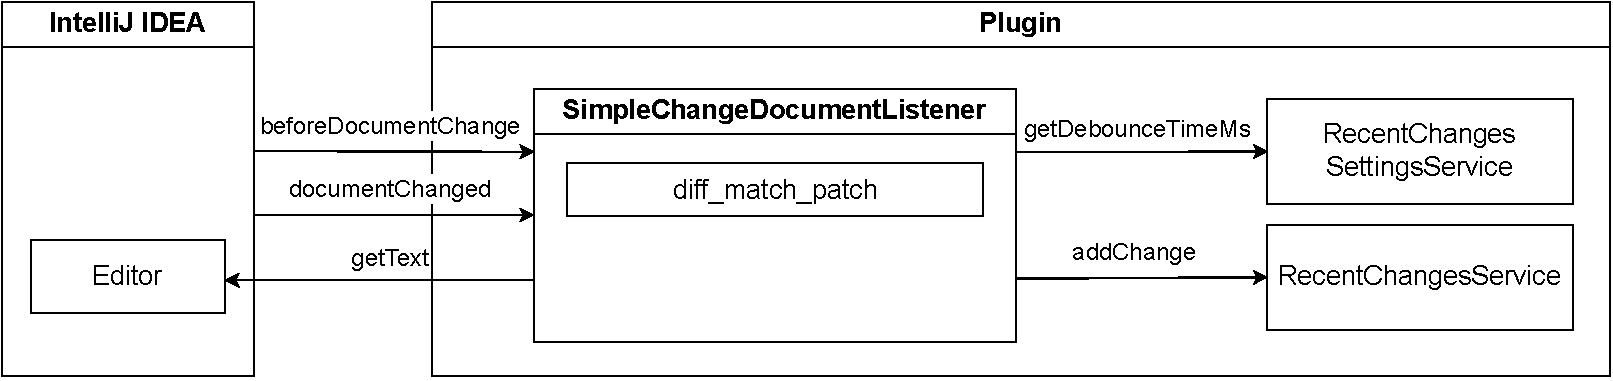
\includegraphics[width=.95\textwidth]{diagram_IntelliJDesign-Detail_Listener}
    \caption{Detaillierte Darstellung des \emph{SimpleChangeDocumentListener}.}
    \label{fig:diagram_IntelliJDesign-Detail_Listener}
\end{figure}   
\begin{figure}
    \centering
    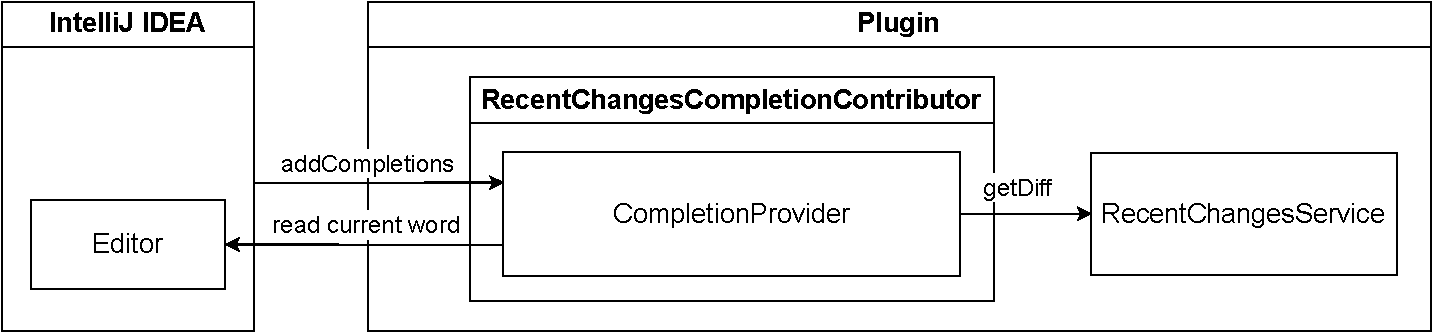
\includegraphics[width=.95\textwidth]{diagram_IntelliJDesign-Detail_Contributor}
    \caption{Detaillierte Darstellung des \emph{RecentChangesCompletionContributor}.}
    \label{fig:diagram_IntelliJDesign-Detail_Contributor}
\end{figure}   
\begin{figure}
    \centering
    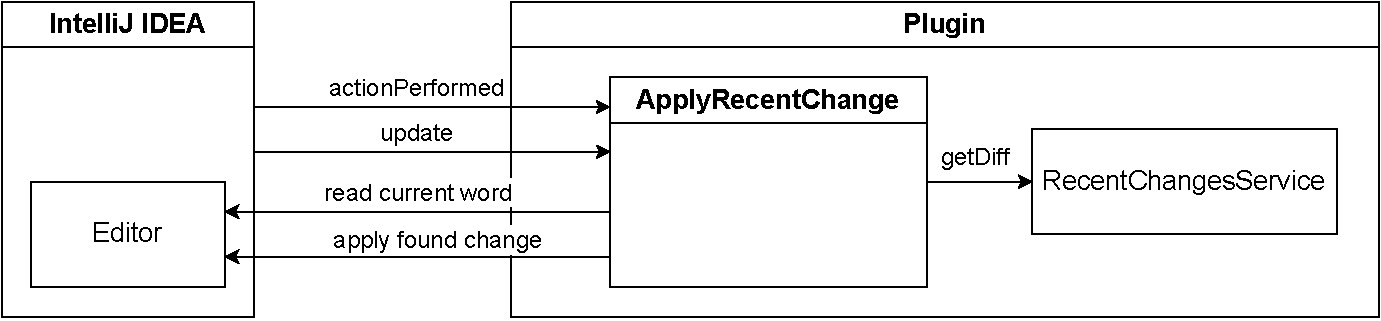
\includegraphics[width=.95\textwidth]{diagram_IntelliJDesign-Detail_Action}
    \caption{Detaillierte Darstellung des Commands \emph{ApplyRecentChange}.}
    \label{fig:diagram_IntelliJDesign-Detail_Action}
\end{figure}   
\begin{figure}
    \centering
    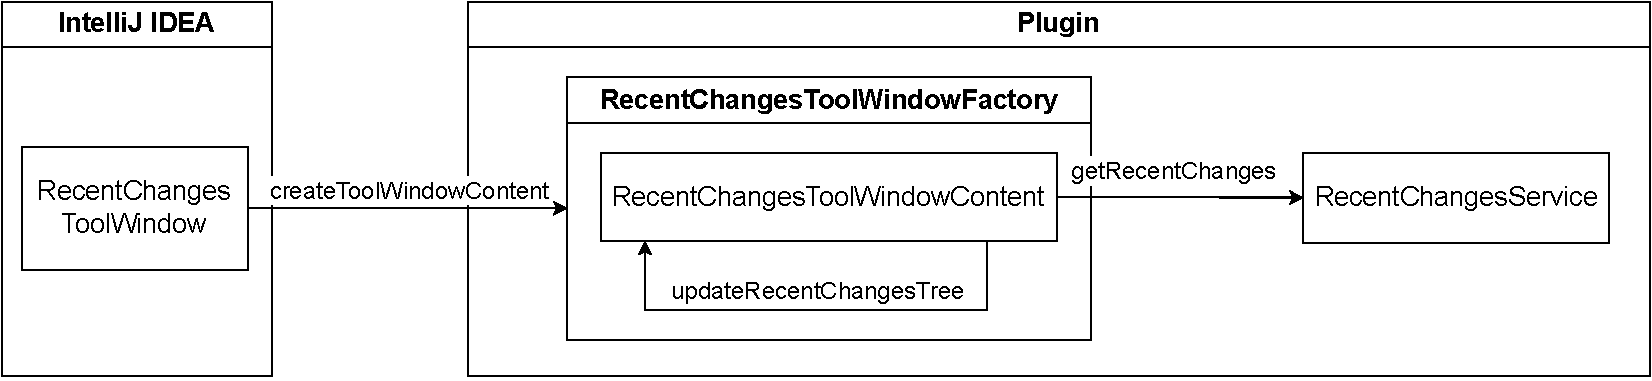
\includegraphics[width=.95\textwidth]{diagram_IntelliJDesign-Detail_ToolWindow}
    \caption{Detaillierte Darstellung der \emph{RecentChangesToolWindowFactory}.}
    \label{fig:diagram_IntelliJDesign-Detail_ToolWindow}
\end{figure}   
\begin{figure}
    \centering
    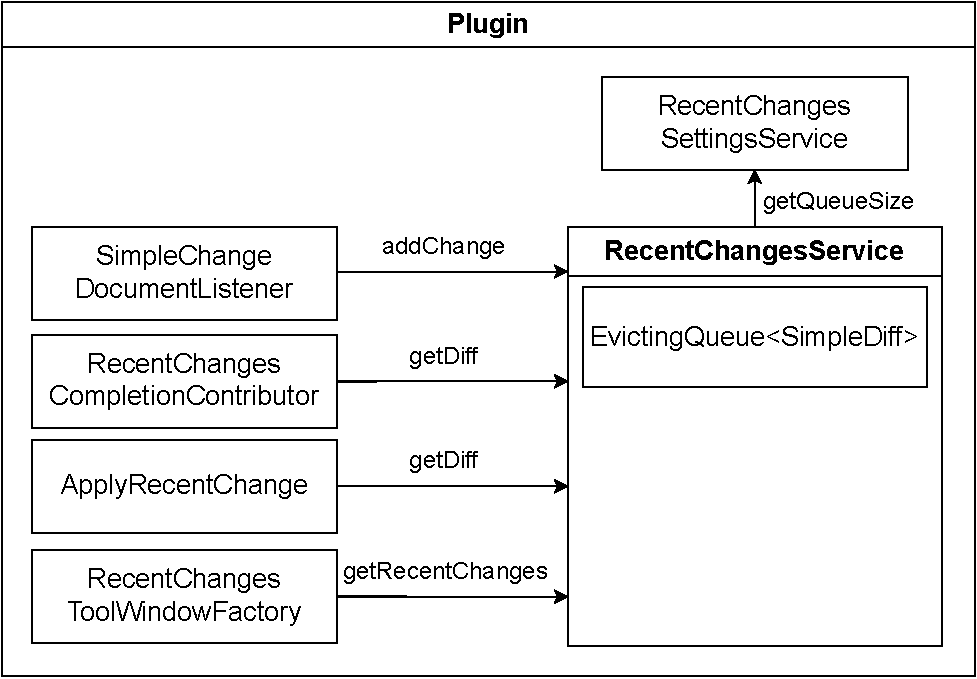
\includegraphics[width=.95\textwidth]{diagram_IntelliJDesign-Detail_Service}
    \caption{Detaillierte Darstellung des \emph{RecentChangesService}.}
    \label{fig:diagram_IntelliJDesign-Detail_Service}
\end{figure}   

\section{Implementierung}
\label{sec:EntwicklungIntelliJ_Implementierung}

\subsection{Aufsetzen des Projektes}

\subsubsection{Aufbau der Ordnerstruktur}

\subsection{Entwicklung}

\section{Tests}
\label{sec:EntwicklungIntelliJ_Tests}

\section{Publishing}
\label{sec:EntwicklungIntelliJ_Publishing}

\section{CI/CD}
\label{sec:EntwicklungIntelliJ_CICD}